\documentclass[3p,times]{elsarticle}

\usepackage[utf8]{inputenc}
\usepackage[T1]{fontenc}
\usepackage{amsmath,amssymb,amsthm}
\usepackage{algorithm}
\usepackage{algpseudocode}
\usepackage{tikz}
\usetikzlibrary{calc,patterns,decorations.pathmorphing,arrows.meta,positioning}
\usepackage{xcolor}
\usepackage{hyperref}
\usepackage{cleveref}

\newtheorem{theorem}{Theorem}
\newtheorem{lemma}[theorem]{Lemma}
\newtheorem{corollary}[theorem]{Corollary}
\newtheorem{proposition}[theorem]{Proposition}
\theoremstyle{definition}
\newtheorem{definition}[theorem]{Definition}
\newtheorem{remark}[theorem]{Remark}

\definecolor{polyblue}{RGB}{70,130,180}
\definecolor{diagred}{RGB}{180,60,60}
\definecolor{chaingreen}{RGB}{60,140,60}

\journal{Computational Geometry: Theory and Applications}

\begin{document}

\begin{frontmatter}

\title{Practical polygonal triangulation in $O(n + r\log r)$ Time}

\author[knu]{Pavel Shpagin\corref{cor1}}
\ead{pavelandrewshpagin@knu.ua}
\author[knu]{Vasyl Tereschenko}
\cortext[cor1]{Corresponding author}
\address[knu]{Faculty of Computer Science and Cybernetics, Taras Shevchenko National University of Kyiv, Kyiv, Ukraine}

\begin{abstract}
We present an algorithm for triangulating a simple polygon with $n$ vertices in $O(n + r\log r)$ time, where $r$ is the number of reflex vertices. The key observation is that a polygon with $r$ reflex vertices has at most $2r+2$ local extrema, enabling a chain-based reformulation of monotone decomposition where the sweep processes $O(r)$ events rather than $O(n)$. Regular vertices are handled via lazy pointer advancement in $O(n)$ amortized time. For $r = o(n/\log n)$, this improves upon the classical $O(n\log n)$ bound while remaining practical to implement.
\end{abstract}

\begin{keyword}
simple polygon \sep triangulation \sep monotone decomposition \sep output-sensitive algorithm \sep plane sweep
\end{keyword}

\end{frontmatter}

%==============================================================================
\section{Introduction}
\label{sec:intro}
%==============================================================================

Triangulating simple polygons is a fundamental problem in computational geometry. Chazelle~\cite{chazelle1991} proved that $O(n)$ time is achievable, but the algorithm's complexity has limited practical adoption. The plane sweep of Garey et al.~\cite{garey1978}, running in $O(n\log n)$ time via monotone decomposition, remains standard; see de Berg et al.~\cite{deberg2008}. Seidel~\cite{seidel1991} gave a randomized $O(n\log^* n)$ expected-time algorithm.

We present an algorithm running in $O(n + r\log r)$ time, where $r$ is the number of \emph{reflex vertices} (interior angle $> \pi$). This interpolates between $O(n)$ for convex polygons ($r = 0$) and $O(n\log n)$ for worst-case polygons ($r = \Theta(n)$), improving upon classical methods when $r = o(n/\log n)$.

The key observation is that a polygon with $r$ reflex vertices has at most $2r + 2$ local extrema (\Cref{lem:extrema}), hence at most $2r + 2$ monotone chains. We reformulate the plane sweep to maintain chains rather than edges: the sweep processes $O(r)$ extrema events with $O(\log r)$ BST operations each, while regular vertices are handled via lazy pointer advancement in $O(n)$ amortized time.

\paragraph{Related work.}
The triangulation problem has a rich history spanning four decades. The earliest approaches include the ear-clipping method of ElGindy et al.~\cite{elgindy1985}, which runs in $O(n^2)$ time. Garey et al.~\cite{garey1978} achieved $O(n \log n)$ time through monotone decomposition, which remains the standard practical approach; see de Berg et al.~\cite{deberg2008} for a textbook treatment. Hertel and Mehlhorn~\cite{hertel1983} provided an alternative $O(n \log n)$ sweep-line algorithm with improved constant factors.

Subsequent work focused on reducing the $O(n \log n)$ bound. Tarjan and Van Wyk~\cite{tarjan1988} achieved $O(n \log \log n)$ using sophisticated data structures, later simplified by Kirkpatrick et al.~\cite{kirkpatrick1992}. Randomized approaches proved fruitful: Clarkson et al.~\cite{clarkson1989} gave an $O(n \log^* n)$ expected-time Las Vegas algorithm, which Seidel~\cite{seidel1991} simplified significantly using trapezoidal decomposition. Amato et al.~\cite{amato2001} provided further simplifications of randomized linear-time triangulation.

The breakthrough came with Chazelle's~\cite{chazelle1991} deterministic $O(n)$ algorithm, resolving a long-standing open problem. However, the algorithm's complexity---involving hierarchical polygon decomposition and intricate merge operations---has limited practical adoption. Fournier and Montuno~\cite{fournier1984} studied triangulation of monotone polygons. Keil~\cite{keil2000} surveys polygon decomposition more broadly. Output-sensitive algorithms exist for related problems: Kirkpatrick and Seidel~\cite{kirkpatrick1986} gave an $O(n \log h)$ convex hull algorithm where $h$ is the output size. Chazelle and Incerpi~\cite{chazelle1984} studied shape complexity and triangulation.

Our work contributes an $O(n + r \log r)$ algorithm that interpolates between these bounds based on polygon complexity. This output-sensitive approach---where $r$ measures input ``difficulty''---appears not to have been previously explored for triangulation, despite its naturalness.

\paragraph{Organization.}
\Cref{sec:prelim} proves the extrema bound. \Cref{sec:algorithm} presents the algorithm. \Cref{sec:correctness} establishes correctness. \Cref{sec:complexity} analyzes complexity. \Cref{sec:experiments} provides experimental evaluation. \Cref{sec:discussion} discusses extensions.

%==============================================================================
\section{Preliminaries}
\label{sec:prelim}
%==============================================================================

Let $P$ be a simple polygon with vertices $v_0, v_1, \ldots, v_{n-1}$ listed in counterclockwise order along the boundary $\partial P$. We write $v_i = (x_i, y_i)$ for the coordinates of each vertex and adopt the convention that indices are taken modulo $n$, so $v_{-1} = v_{n-1}$ and $v_n = v_0$. The \emph{interior angle} at vertex $v_i$ is the angle $\angle v_{i-1} v_i v_{i+1}$ measured inside $P$. A vertex is \emph{convex} if its interior angle is at most $\pi$ and \emph{reflex} if its interior angle strictly exceeds $\pi$. We denote by $r$ the number of reflex vertices.

\begin{definition}[Vertex classification]
\label{def:vertex-types}
Assuming general position (no two vertices share the same $y$-coordinate), each vertex $v_i$ is classified according to the relative $y$-coordinates of its neighbors:
\begin{itemize}
\item \textbf{Start vertex:} $y_{i-1} < y_i$ and $y_{i+1} < y_i$, with interior angle $< \pi$.
\item \textbf{Split vertex:} $y_{i-1} < y_i$ and $y_{i+1} < y_i$, with interior angle $> \pi$.
\item \textbf{End vertex:} $y_{i-1} > y_i$ and $y_{i+1} > y_i$, with interior angle $< \pi$.
\item \textbf{Merge vertex:} $y_{i-1} > y_i$ and $y_{i+1} > y_i$, with interior angle $> \pi$.
\item \textbf{Regular vertex:} exactly one neighbor has $y$-coordinate greater than $y_i$.
\end{itemize}
\end{definition}

Start and split vertices are \emph{local maxima}; end and merge vertices are \emph{local minima}. Split and merge vertices are precisely the reflex vertices among local extrema. Regular vertices partition into two subtypes based on whether the polygon interior lies to their left or right as one traverses the boundary; this distinction, while important for implementation, does not affect our analysis.

\begin{definition}[Monotone chain]
\label{def:chain}
A \emph{$y$-monotone chain} is a maximal contiguous sequence of boundary vertices $v_a, v_{a+1}, \ldots, v_b$ such that the $y$-coordinates are strictly monotonic (either strictly increasing or strictly decreasing) along the sequence. Each chain connects a local maximum to a local minimum.
\end{definition}

The boundary $\partial P$ decomposes uniquely into monotone chains, with consecutive chains sharing their endpoint extrema. If there are $k$ local maxima, there are also $k$ local minima (since the boundary is a closed curve), and hence $2k$ chains. The following lemma bounds $k$ in terms of $r$.

\begin{lemma}[Extrema bound]
\label{lem:extrema}
A simple polygon with $r$ reflex vertices has at most $r + 1$ local maxima, and hence at most $2r + 2$ local extrema and $2r + 2$ monotone chains.
\end{lemma}

\begin{proof}
Let $k$ denote the number of local maxima, which equals the number of local minima (since the boundary is a closed curve that alternates between ascending and descending). Among local maxima, let $s$ denote the number of \emph{split vertices} (reflex); among local minima, let $m$ denote the number of \emph{merge vertices} (reflex). The remaining $k - s$ local maxima are \emph{start vertices} (convex), and the remaining $k - m$ local minima are \emph{end vertices} (convex). Since split and merge vertices are reflex, $s + m \leq r$.

We establish $k \leq r + 1$ by constructing an injection from start vertices (except possibly one) to merge vertices.

\medskip
\noindent\textbf{Construction.} Order all local maxima by decreasing $y$-coordinate: $M_1, M_2, \ldots, M_k$. For $i \in \{1, \ldots, k-1\}$, define the \emph{horizontal slab}
\[
H_i = \bigl\{(x,y) : y_{M_{i+1}} < y < y_{M_i}\bigr\}.
\]
Since $M_i$ and $M_{i+1}$ are consecutive in $y$-order, no local maximum lies in $H_i$.

\medskip
\noindent\textbf{Slab occupancy.} From each local maximum $M_i$, two boundary paths descend (the edges at a local maximum both go downward). Each path must reach a local minimum before ascending to another maximum. For $i < k$, let $\nu_i$ be the first local minimum reached by either descending path from $M_i$. We claim $\nu_i \in H_i$.

\emph{Proof:} Suppose $y_{\nu_i} \leq y_{M_{i+1}}$. Then the descending path from $M_i$ to $\nu_i$ drops below height $y_{M_{i+1}}$. After $\nu_i$, the path ascends toward another maximum. The next maximum on this path has $y$-coordinate at least $y_{\nu_i}$'s successor maximum in $y$-order. But $M_{i+1}$ is the next maximum below $M_i$, and we assumed $\nu_i$ lies at or below $M_{i+1}$. For the boundary to close, the ascending path from $\nu_i$ must reach some maximum. If that maximum were $M_{i+1}$ or higher, the path would have to pass through $H_i$ while ascending, meaning $\nu_i$ must be in $H_i$ after all. Contradiction. Hence $y_{\nu_i} > y_{M_{i+1}}$, so $\nu_i \in H_i$. $\diamond$

\medskip
\noindent\textbf{Key claim:} \emph{If $M_i$ is a start vertex (convex local maximum), then $\nu_i$ is a merge vertex (reflex local minimum).}

\emph{Proof of claim:} Let $M_i = v_j$ in the polygon's vertex ordering. At start vertex $M_i$, the interior angle $\angle v_{j-1} v_j v_{j+1} < \pi$. Orient $\partial P$ counterclockwise. The two edges at $M_i$ are $e^- = \overrightarrow{v_{j-1} v_j}$ (incoming) and $e^+ = \overrightarrow{v_j v_{j+1}}$ (outgoing), both ascending to $M_i$ then descending.

Since the interior angle is convex, when standing at $M_i$ and looking along the outgoing edge $e^+$, the polygon interior lies to the \emph{left}. Equivalently, the interior lies in the half-plane $\mathcal{H}^+$ to the left of the line through $e^+$. The key observation is that at $M_i$, the two descending edges ``spread apart'' with the interior between them---the boundary forms a convex cap over the interior.

Now trace the boundary path $\gamma$ that follows $e^+$ downward from $M_i$. This path eventually reaches $\nu_i$, the first local minimum. At $\nu_i = v_\ell$, two edges ascend: $e_1 = \overrightarrow{v_{\ell-1} v_\ell}$ (incoming) and $e_2 = \overrightarrow{v_\ell v_{\ell+1}}$ (outgoing).

Consider the simple closed curve $\Gamma$ formed by:
\begin{enumerate}
    \item[(i)] the boundary path from $M_i$ to $\nu_i$ via $\gamma$, and
    \item[(ii)] the vertical segment from $\nu_i$ up to the horizontal line $y = y_{M_i}$, then horizontally to $M_i$.
\end{enumerate}
(We use a slight perturbation to ensure $\Gamma$ is simple if needed.)

By the Jordan curve theorem, $\Gamma$ partitions the plane into two regions. The polygon interior $\mathrm{int}(P)$ intersects the region ``inside'' this curve (on the left side of $\gamma$ as traced from $M_i$ to $\nu_i$, since $P$ is CCW-oriented).

At $\nu_i$, the boundary path $\gamma$ has been descending (from $M_i$) and now the edges $e_1, e_2$ ascend. For the polygon to close correctly:
\begin{itemize}
    \item The interior of $P$ lies to the left of $\gamma$ throughout the descent.
    \item At $\nu_i$, the interior must still lie to the left of the outgoing direction.
    \item The two ascending edges $e_1, e_2$ must therefore bend \emph{inward} (toward the region containing the interior traced so far).
\end{itemize}

Formally, the signed curvature of the boundary at $\nu_i$ has the opposite sign from that at $M_i$. At start $M_i$, the boundary curves \emph{away} from the interior (exterior curvature). At $\nu_i$, to maintain the interior on the left while transitioning from descending to ascending, the boundary must curve \emph{toward} the interior (interior curvature). This requires interior angle $\angle v_{\ell-1} v_\ell v_{\ell+1} > \pi$, making $\nu_i$ a merge vertex. $\diamondsuit$

\medskip
\noindent\textbf{Injection.} Define $\phi: \{\text{starts among } M_1, \ldots, M_{k-1}\} \to \{\text{merges}\}$ by $\phi(M_i) = \nu_i$. By the claim, $\phi$ is well-defined. Since slabs $H_1, \ldots, H_{k-1}$ are pairwise disjoint and each $\nu_i \in H_i$, the map $\phi$ is injective: distinct starts map to distinct merges.

Thus $|\{M_i : i < k, M_i \text{ is a start}\}| \leq m$.

\medskip
\noindent\textbf{Counting.} Let $s'$ denote the number of starts among $M_1, \ldots, M_{k-1}$. Then:
\begin{itemize}
    \item Total starts: $(k - s) = s' + \mathbf{1}[M_k \text{ is a start}] \leq s' + 1$.
    \item From injection: $s' \leq m$.
\end{itemize}
Hence $(k - s) \leq m + 1$, giving
\[
k = s + (k - s) \leq s + (m + 1) = (s + m) + 1 \leq r + 1.
\]
Total local extrema: $2k \leq 2r + 2$. Total monotone chains: $2k \leq 2r + 2$.
\end{proof}

\begin{remark}[Tightness]
The bound is achieved by staircase polygons. A staircase with $t$ ``steps'' has $t$ reflex vertices (alternating between splits ascending and merges descending) and $t + 1$ local maxima.
\end{remark}

\begin{figure}[t]
\centering
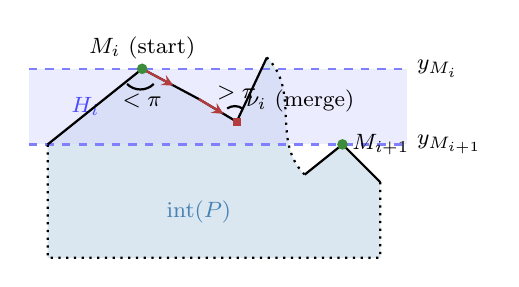
\begin{tikzpicture}[scale=0.48, every node/.style={font=\footnotesize}]
% Illustration of Lemma proof: start -> merge injection
% Design: M_i and M_{i+1} are on DIFFERENT descending branches from the polygon
% The path shown descends from M_i to nu_i; M_{i+1} is on another branch

% Left branch: descends from M_i to nu_i
\coordinate (p1) at (0, 4);        % approaching M_i from below-left
\coordinate (M1) at (2.5, 6);      % M_i - start vertex (local max)
\coordinate (p2) at (4, 5.2);      % descending from M_i
\coordinate (nu) at (5, 4.6);      % nu_i - merge vertex (local min)
\coordinate (p3) at (5.8, 6.3);    % ascending from nu - ABOVE slab (any local max here is M_{j<i})

% Right branch: M_{i+1} on separate descending path
\coordinate (q1) at (6.8, 3.2);    % neighbor of M_{i+1} (below)
\coordinate (M2) at (7.8, 4);      % M_{i+1} - next local max in y-order
\coordinate (q2) at (8.8, 3);      % neighbor of M_{i+1} (below)

% Interior indication (polygon interior is below/inside the boundary)
\fill[polyblue!20] (p1) -- (M1) -- (p2) -- (nu) -- (p3) 
    to[out=-45, in=135] (q1) -- (M2) -- (q2) 
    -- (8.8, 1) -- (0, 1) -- cycle;
\node[polyblue] at (4, 2.2) {$\mathrm{int}(P)$};

% Slab H_i: between y_{M_{i+1}}=4 and y_{M_i}=6 (transparent overlay)
\fill[blue!15, opacity=0.5] (-0.5, 4) rectangle (9.5, 6);
\draw[blue!50, thick, dashed] (-0.5, 6) -- (9.5, 6) node[right, black] {$y_{M_i}$};
\draw[blue!50, thick, dashed] (-0.5, 4) -- (9.5, 4) node[right, black] {$y_{M_{i+1}}$};
\node[blue!70] at (1, 5) {$H_i$};

% Boundary path: p1 -> M_i -> p2 -> nu -> p3
\draw[thick] (p1) -- (M1) -- (p2) -- (nu) -- (p3);

% Descent arrows from M_i
\draw[thick, diagred, ->, >=stealth] (M1) -- ($(M1)!0.55!(p2)$);
\draw[thick, diagred, ->, >=stealth] (p2) -- ($(p2)!0.65!(nu)$);

% Dotted continuation: boundary curves down (p3 is above slab, any max there is M_{j<i})
\draw[thick, dotted] (p3) to[out=-45, in=135] (q1);

% Boundary path: q1 -> M_{i+1} -> q2
\draw[thick] (q1) -- (M2) -- (q2);

% Dotted closure at bottom
\draw[thick, dotted] (q2) -- (8.8, 1) -- (0, 1) -- (p1);

% Vertices
\fill[chaingreen] (M1) circle (4pt);
\node[above] at (M1) {$M_i$ (start)};
\fill[chaingreen] (M2) circle (4pt);
\node[right] at (M2) {$M_{i+1}$};
\fill[diagred] (nu) ++(-3pt,-3pt) rectangle ++(6pt, 6pt);
\node[above right] at (nu) {$\nu_i$ (merge)};

% Angle indicators
\draw[thick] ($(M1)+(-0.4, -0.4)$) arc[start angle=225, end angle=315, radius=0.5];
\node at ($(M1)+(0, -0.85)$) {$<\pi$};
\draw[thick] ($(nu)+(-0.25, 0.35)$) arc[start angle=125, end angle=55, radius=0.35];
\node at ($(nu)+(0, 0.75)$) {$>\pi$};

\end{tikzpicture}
\caption{Illustration of \Cref{lem:extrema}: from start vertex $M_i$ (convex local maximum, interior angle $< \pi$), the boundary descends to merge vertex $\nu_i$ (reflex local minimum, interior angle $> \pi$) within slab $H_i$. The dotted curve indicates the boundary continues (potentially through other local extrema outside the slab) to reach $M_{i+1}$, the next local maximum below $M_i$ in $y$-order.}
\label{fig:lemma-proof}
\end{figure}

%==============================================================================
\section{Algorithm}
\label{sec:algorithm}
%==============================================================================

The algorithm consists of three phases: (1) chain construction and vertex classification, (2) monotone decomposition via chain-based plane sweep, and (3) triangulation of monotone pieces. We describe each phase in detail.

%------------------------------------------------------------------------------
\subsection{Phase 1: Chain Construction}
\label{sec:chain-construction}
%------------------------------------------------------------------------------

A single traversal of $\partial P$ classifies each vertex according to \Cref{def:vertex-types} and partitions the boundary into monotone chains. For each vertex $v_i$, we compare $y_i$ to $y_{i-1}$ and $y_{i+1}$ and compute the cross product $(v_{i+1} - v_i) \times (v_i - v_{i-1})$ to determine convexity. Simultaneously, we record each chain as an array of vertex indices from its upper endpoint (local maximum) to its lower endpoint (local minimum). For each local minimum $v$, we store a pointer to the unique \emph{left-boundary chain} terminating at $v$---the chain for which, when traversed from upper to lower endpoint, the polygon interior lies to the right.

\begin{definition}[Left-boundary chain]
\label{def:left-boundary}
A monotone chain is a \emph{left-boundary chain} if, when traversed from its upper endpoint to its lower endpoint, the polygon interior lies to the right of the traversal direction. Equivalently, for a counterclockwise-oriented polygon, a chain is left-boundary if its traversal direction (downward) opposes the boundary orientation.
\end{definition}

At each local maximum, exactly one of the two originating chains is left-boundary; at each local minimum, exactly one of the two terminating chains is left-boundary. This phase runs in $O(n)$ time and produces $O(r)$ chains.

%------------------------------------------------------------------------------
\subsection{Phase 2: Monotone Decomposition}
\label{sec:decomposition}
%------------------------------------------------------------------------------

A polygon is \emph{$y$-monotone} if every horizontal line intersects it in a connected set (either empty, a point, or a segment). Split vertices violate monotonicity by creating local maxima where the boundary diverges downward; merge vertices violate it by creating local minima where boundary paths converge from above. The decomposition phase inserts diagonals to eliminate all split and merge vertices, partitioning $P$ into $y$-monotone subpolygons.

\paragraph{Sweep-line status structure.}
Unlike the classical algorithm, which maintains individual edges in a balanced search tree $T$, we maintain \emph{active left-boundary chains}. A chain $C$ is \emph{active} at sweep height $y$ if $y$ lies strictly between the $y$-coordinates of $C$'s upper and lower endpoints. The tree $T$ stores active left-boundary chains ordered by their $x$-coordinate at the current sweep height.

Each chain $C$ in $T$ maintains:
\begin{enumerate}
\item \textbf{Edge pointer} $C.\mathit{curr}$: initialized to the topmost edge of $C$, this pointer tracks our position within the chain. The upper vertex of $C.\mathit{curr}$ serves as the \emph{slab entry}---the default diagonal target when no pending merge exists.
\item \textbf{Pending merge} $C.\mathit{pending}$: either null or a merge vertex awaiting connection to a lower vertex. When a merge vertex $v$ is processed and $C$ is immediately to $v$'s left, we set $C.\mathit{pending} \gets v$.
\end{enumerate}

\paragraph{Lazy edge pointer advancement.}
The comparison function for $T$, when comparing chains at sweep height $y$, first advances each chain's edge pointer to ensure the current edge spans $y$:
\begin{algorithmic}[1]
\Procedure{Advance}{$C, y$}
    \While{$C.\mathit{curr}.\mathit{lower}.y > y$}
        \State $C.\mathit{curr} \gets$ next edge down $C$
    \EndWhile
\EndProcedure
\end{algorithmic}
After advancement, the $x$-coordinate of $C$ at height $y$ is computed by linear interpolation along $C.\mathit{curr}$. Since each vertex is visited by at most one chain's pointer exactly once, the total cost of all pointer advancements is $O(n)$, amortized over all tree operations.

\paragraph{Event processing.}
The sweep processes local extrema in decreasing $y$-order. Let $E$ denote the sorted list of extrema; $|E| \leq 2r + 2$ by \Cref{lem:extrema}.

\begin{algorithm}[t]
\caption{Chain-Based Monotone Decomposition}
\label{alg:decompose}
\begin{algorithmic}[1]
\Require Polygon $P$ with classified vertices and identified left-boundary chains
\Ensure Diagonal set $D$ partitioning $P$ into $y$-monotone subpolygons
\State $E \gets$ local extrema sorted by decreasing $y$-coordinate
\State $T \gets$ empty balanced BST of active left-boundary chains
\State $D \gets \emptyset$
\For{each extremum $v$ in $E$}
    \Switch{type of $v$}
        \Case{Start}
            \State Insert left-boundary chain originating at $v$ into $T$
            \State Initialize $C.\mathit{curr}$ to top edge, $C.\mathit{pending} \gets \textsc{null}$
        \EndCase
        \Case{End}
            \State $R \gets$ left-boundary chain terminating at $v$
            \If{$R.\mathit{pending} \neq \textsc{null}$}
                \State $D \gets D \cup \{(v, R.\mathit{pending})\}$ \Comment{Connect pending merge downward}
            \EndIf
            \State Remove $R$ from $T$
        \EndCase
        \Case{Split}
            \State $L \gets$ predecessor of $v$ in $T$ \Comment{Chain immediately left of $v$}
            \If{$L.\mathit{pending} \neq \textsc{null}$}
                \State $D \gets D \cup \{(v, L.\mathit{pending})\}$; $L.\mathit{pending} \gets \textsc{null}$
            \Else
                \State $D \gets D \cup \{(v, L.\mathit{curr}.\mathit{upper})\}$ \Comment{Slab entry}
            \EndIf
            \State Insert left-boundary chain originating at $v$ into $T$
        \EndCase
        \Case{Merge}
            \State $R \gets$ left-boundary chain terminating at $v$
            \State $L \gets$ predecessor of $R$ in $T$ \Comment{Chain immediately left}
            \If{$R.\mathit{pending} \neq \textsc{null}$}
                \State $D \gets D \cup \{(v, R.\mathit{pending})\}$
            \EndIf
            \If{$L.\mathit{pending} \neq \textsc{null}$}
                \State $D \gets D \cup \{(v, L.\mathit{pending})\}$
            \EndIf
            \State $L.\mathit{pending} \gets v$
            \State Remove $R$ from $T$
        \EndCase
    \EndSwitch
\EndFor
\State \Return $D$
\end{algorithmic}
\end{algorithm}

The complete decomposition procedure is given in \Cref{alg:decompose}. For split vertices, we connect upward to either a pending merge (if one exists on the immediately-left chain) or to the slab entry (the upper vertex of the current edge on that chain). For merge vertices, we first resolve any pending merges on both the terminating chain and the chain to its left, then register the current vertex as pending on the left chain.

%------------------------------------------------------------------------------
\subsection{Phase 3: Triangulation}
\label{sec:triangulation}
%------------------------------------------------------------------------------

The diagonals from Phase 2 partition $P$ into $y$-monotone subpolygons. We construct a doubly-connected edge list (DCEL) or equivalent adjacency structure from the original boundary edges plus the $|D| \leq r$ diagonals. Each face is extracted by traversing half-edges, yielding the vertex sequence of each monotone subpolygon. 

Each $y$-monotone polygon with $m$ vertices is triangulated in $O(m)$ time using the classical stack-based algorithm: vertices are processed in $y$-sorted order, maintaining a stack representing the ``reflex chain'' of vertices not yet triangulated. When a vertex from the opposite chain is encountered, all stack vertices are triangulated; when a vertex from the same chain is encountered, we triangulate as many stack vertices as remain visible. Since the sum of face sizes equals $n + 2|D| = O(n)$, the total triangulation time is $O(n)$.

%------------------------------------------------------------------------------
\subsection{Illustrative Example}
\label{sec:example}
%------------------------------------------------------------------------------

\begin{figure*}[t]
\centering
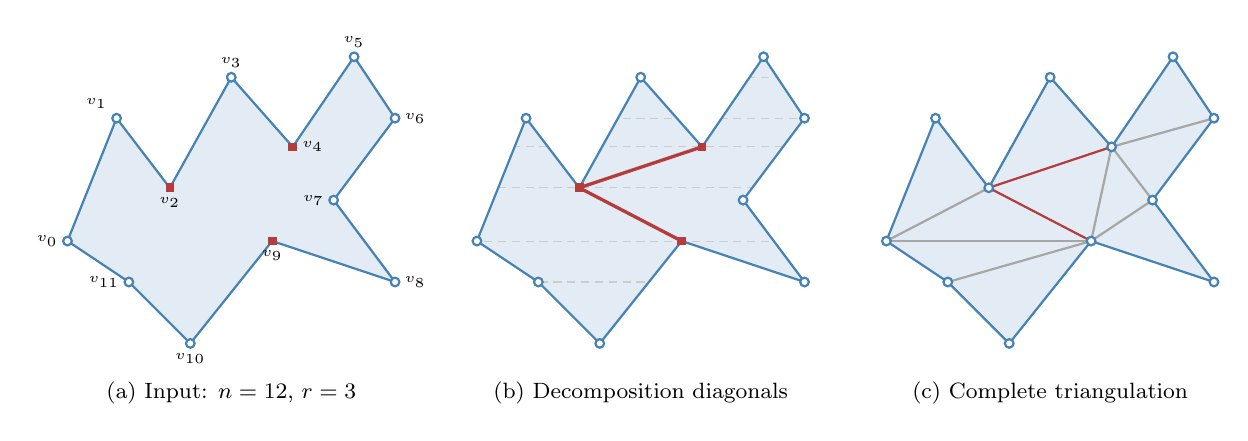
\begin{tikzpicture}[scale=0.52, every node/.style={font=\footnotesize}]

% Polygon vertices - defined globally
\coordinate (v0) at (0, 2.5);
\coordinate (v1) at (1.2, 5.5);
\coordinate (v2) at (2.5, 3.8);
\coordinate (v3) at (4, 6.5);
\coordinate (v4) at (5.5, 4.8);
\coordinate (v5) at (7, 7);
\coordinate (v6) at (8, 5.5);
\coordinate (v7) at (6.5, 3.5);
\coordinate (v8) at (8, 1.5);
\coordinate (v9) at (5, 2.5);
\coordinate (v10) at (3, 0);
\coordinate (v11) at (1.5, 1.5);

\def\polygon{(v0) -- (v1) -- (v2) -- (v3) -- (v4) -- (v5) -- (v6) -- (v7) -- (v8) -- (v9) -- (v10) -- (v11) -- cycle}

% (a) Input polygon
\begin{scope}[xshift=0cm]
    \fill[polyblue!15] \polygon;
    \draw[polyblue, thick] \polygon;
    
    % Convex vertices: circles
    \foreach \v in {v0,v1,v3,v5,v6,v7,v8,v10,v11} {
        \fill[white] (\v) circle (3pt);
        \draw[polyblue, thick] (\v) circle (3pt);
    }
    % Reflex vertices: squares
    \foreach \v in {v2,v4,v9} {
        \fill[diagred] (\v) ++(-3pt,-3pt) rectangle ++(6pt,6pt);
    }
    
    % Labels
    \node[left, font=\tiny] at (v0) {$v_0$};
    \node[above left, font=\tiny] at (v1) {$v_1$};
    \node[below, font=\tiny] at (v2) {$v_2$};
    \node[above, font=\tiny] at (v3) {$v_3$};
    \node[right, font=\tiny] at (v4) {$v_4$};
    \node[above, font=\tiny] at (v5) {$v_5$};
    \node[right, font=\tiny] at (v6) {$v_6$};
    \node[left, font=\tiny] at (v7) {$v_7$};
    \node[right, font=\tiny] at (v8) {$v_8$};
    \node[below, font=\tiny] at (v9) {$v_9$};
    \node[below, font=\tiny] at (v10) {$v_{10}$};
    \node[left, font=\tiny] at (v11) {$v_{11}$};
    
    \node at (4, -1.2) {(a) Input: $n=12$, $r=3$};
\end{scope}

% (b) Monotone decomposition with diagonals
\begin{scope}[xshift=10cm]
    % Redefine coordinates for this scope
    \coordinate (v0) at (0, 2.5);
    \coordinate (v1) at (1.2, 5.5);
    \coordinate (v2) at (2.5, 3.8);
    \coordinate (v3) at (4, 6.5);
    \coordinate (v4) at (5.5, 4.8);
    \coordinate (v5) at (7, 7);
    \coordinate (v6) at (8, 5.5);
    \coordinate (v7) at (6.5, 3.5);
    \coordinate (v8) at (8, 1.5);
    \coordinate (v9) at (5, 2.5);
    \coordinate (v10) at (3, 0);
    \coordinate (v11) at (1.5, 1.5);
    
    \fill[polyblue!15] \polygon;
    
    % Sweep lines at extrema heights (clipped to polygon)
    \begin{scope}
        \clip \polygon;
        \foreach \y in {7, 6.5, 5.5, 4.8, 3.8, 2.5, 1.5, 0} {
            \draw[gray!40, densely dashed, thin] (-0.5, \y) -- (8.5, \y);
        }
    \end{scope}
    
    \draw[polyblue, thick] \polygon;
    
    % Decomposition diagonals (bold red)
    \draw[diagred, very thick] (v2) -- (v4);
    \draw[diagred, very thick] (v9) -- (v2);
    
    % Vertices
    \foreach \v in {v0,v1,v3,v5,v6,v7,v8,v10,v11} {
        \fill[white] (\v) circle (3pt);
        \draw[polyblue, thick] (\v) circle (3pt);
    }
    \foreach \v in {v2,v4,v9} {
        \fill[diagred] (\v) ++(-3pt,-3pt) rectangle ++(6pt,6pt);
    }
    
    \node at (4, -1.2) {(b) Decomposition diagonals};
\end{scope}

% (c) Final triangulation
\begin{scope}[xshift=20cm]
    % Redefine coordinates for this scope
    \coordinate (v0) at (0, 2.5);
    \coordinate (v1) at (1.2, 5.5);
    \coordinate (v2) at (2.5, 3.8);
    \coordinate (v3) at (4, 6.5);
    \coordinate (v4) at (5.5, 4.8);
    \coordinate (v5) at (7, 7);
    \coordinate (v6) at (8, 5.5);
    \coordinate (v7) at (6.5, 3.5);
    \coordinate (v8) at (8, 1.5);
    \coordinate (v9) at (5, 2.5);
    \coordinate (v10) at (3, 0);
    \coordinate (v11) at (1.5, 1.5);

    \fill[polyblue!15] \polygon;
    \draw[polyblue, thick] \polygon;
    
    % Decomposition diagonals
    \draw[diagred, thick] (v2) -- (v4);
    \draw[diagred, thick] (v9) -- (v2);
    
    % Triangulation diagonals (gray)
    \draw[gray!70, thick] (v0) -- (v2);
    \draw[gray!70, thick] (v0) -- (v9);
    \draw[gray!70, thick] (v9) -- (v11);
    \draw[gray!70, thick] (v4) -- (v6);
    \draw[gray!70, thick] (v4) -- (v7);
    \draw[gray!70, thick] (v4) -- (v9);
    \draw[gray!70, thick] (v7) -- (v9);
    
    % Vertices
    \foreach \v in {v0,v1,v2,v3,v4,v5,v6,v7,v8,v9,v10,v11} {
        \fill[white] (\v) circle (3pt);
        \draw[polyblue, thick] (\v) circle (3pt);
    }
    
    \node at (4, -1.2) {(c) Complete triangulation};
\end{scope}

\end{tikzpicture}
\caption{Triangulation of a 12-vertex polygon with 3 reflex vertices (squares). (a)~Input polygon $P$; circles denote convex vertices, squares denote reflex vertices $v_2$ (merge), $v_4$ (merge), $v_9$ (split). (b)~Monotone decomposition: dashed lines indicate sweep heights at local extrema; bold diagonals $(v_2, v_4)$ and $(v_9, v_2)$ partition $P$ into three $y$-monotone pieces. (c)~Final triangulation with $n - 2 = 10$ triangles; decomposition diagonals in bold, triangulation diagonals in gray.}
\label{fig:example}
\end{figure*}

\Cref{fig:example} illustrates the algorithm on a polygon with $n = 12$ vertices and $r = 3$ reflex vertices ($v_2$, $v_4$ are merges; $v_9$ is a split). The sweep processes 9 local extrema. At merge $v_4$, the pending mechanism registers $v_4$ on the left chain. At merge $v_2$, the pending $v_4$ triggers diagonal $(v_2, v_4)$, then $v_2$ becomes pending. At split $v_9$, the pending $v_2$ triggers diagonal $(v_9, v_2)$. The two diagonals partition $P$ into three $y$-monotone faces, yielding 10 triangles.

%==============================================================================
\section{Correctness}
\label{sec:correctness}
%==============================================================================

We establish correctness through three claims: (1) every diagonal lies strictly in the polygon interior, (2) no two diagonals cross, and (3) every split and merge vertex is eliminated by a diagonal. The proofs rely on slab-based visibility invariants.

\begin{definition}[Slab]
\label{def:slab}
For a left-boundary chain $L$ active at height $y$, the \emph{slab} of $L$ is the region bounded on the left by $L$, on the right by the next left-boundary chain (or the polygon's rightmost boundary), and vertically by the $y$-range over which this configuration persists.
\end{definition}

\begin{lemma}[Slab convexity]
\label{lem:slab-convex}
Every slab is horizontally convex: any horizontal segment contained in the slab lies entirely in $\mathrm{int}(P)$.
\end{lemma}

\begin{proof}
A slab is bounded on the left by a left-boundary chain $L$ (with $\mathrm{int}(P)$ to its right) and on the right by either another left-boundary chain or the polygon's right boundary. Between consecutive left-boundary chains, the polygon interior forms a horizontally convex region by definition.
\end{proof}

\begin{lemma}[Pending visibility]
\label{lem:pending-vis}
If $L.\mathit{pending} = v$ for some merge vertex $v$, then $v$ lies in the slab of $L$, and for any point $p$ on $L$ with $p.y < v.y$, the segment $vp$ lies in $\mathrm{int}(P)$.
\end{lemma}

\begin{proof}
When merge $v$ is processed, the algorithm sets $L.\mathit{pending} \gets v$ for the chain $L$ immediately to $v$'s left. By construction, $v$ is in the slab of $L$ at height $v.y$. The slab extends downward to $L$'s lower endpoint or until the slab structure changes at the next event. Any point $p$ on $L$ below $v$ lies in the same slab, and by \Cref{lem:slab-convex}, the segment from $v$ horizontally to $L$ lies in $\mathrm{int}(P)$. Since $p.y < v.y$, the segment $vp$ remains within the slab's vertical extent and cannot cross $L$ at an interior point (as $v$ is strictly right of $L$ and $p$ is on $L$). By convexity of the slab in the horizontal direction and the monotonicity of $L$, the segment $vp$ lies entirely in $\mathrm{int}(P)$.
\end{proof}

\begin{lemma}[Slab entry visibility]
\label{lem:entry-vis}
When processing a split or merge vertex $v$ in the slab of chain $L$, let $w = L.\mathit{curr}.\mathit{upper}$ be the slab entry. Then $w.y > v.y$ and the segment $vw$ lies in $\mathrm{int}(P)$.
\end{lemma}

\begin{proof}
By lazy advancement, $L.\mathit{curr}$ spans the current sweep height $v.y$: the upper vertex $w$ satisfies $w.y \geq v.y$ and the lower vertex $w'$ satisfies $w'.y \leq v.y$. Since $v$ is strictly in the interior of the slab (not on $L$), we have $w.y > v.y$ (equality would place $v$ on $L$).

The segment $vw$ goes from $v$ (strictly right of $L$ at height $v.y$) to $w$ (on $L$ at height $w.y > v.y$). We verify $vw$ does not cross $\partial P$:

\begin{itemize}
\item \emph{Chain $L$:} The segment $vw$ has endpoint $w \in L$. At any height $y^* \in (v.y, w.y)$, the segment $vw$ has $x$-coordinate $x_{vw}(y^*) = v.x + (w.x - v.x)(y^* - v.y)/(w.y - v.y)$. Since $v.x > x_L(v.y)$ (as $v$ is right of $L$) and $w.x = x_L(w.y)$, linear interpolation shows $x_{vw}(y^*) > x_L(y^*)$ for $y^* \in (v.y, w.y)$. Thus $vw$ does not cross $L$ except at $w$.

\item \emph{Right boundary of slab:} The segment goes leftward from $v$, away from the right boundary.

\item \emph{Other boundary components:} Any edge of $\partial P$ in the $y$-range $(v.y, w.y)$ not on $L$ or the right boundary of the slab is separated from the slab by a complete chain and cannot be crossed by a segment within the slab.
\end{itemize}

Hence $vw \subset \mathrm{int}(P)$.
\end{proof}

\begin{theorem}[Correctness]
\label{thm:correct}
\Cref{alg:decompose} produces a valid set of non-crossing diagonals partitioning $P$ into $y$-monotone subpolygons.
\end{theorem}

\begin{proof}
\emph{Claim 1: Diagonals lie in $\mathrm{int}(P)$.} Each diagonal $(v, w)$ falls into one of the cases analyzed in Lemmas~\ref{lem:pending-vis} and~\ref{lem:entry-vis}. In all cases, we have established $vw \subset \mathrm{int}(P)$ except at endpoints.

\emph{Claim 2: Diagonals are non-crossing.} Consider distinct diagonals $(a, b)$ and $(c, d)$ with $a.y < b.y$ and $c.y < d.y$. Let $L_a, L_c$ denote their associated left-boundary chains. If $L_a = L_c$, both diagonals emanate from the same chain; the pending mechanism ensures targets are assigned in $y$-decreasing order, creating a non-crossing ``staircase'' pattern. If $L_a \neq L_c$, the diagonals lie in disjoint slabs and cannot intersect.

\emph{Claim 3: All reflex extrema eliminated.} Every split vertex immediately receives an upward diagonal (to pending or slab entry). Every merge vertex $v$ is registered as $L.\mathit{pending}$ and subsequently connected to a lower vertex when: (i) a split or merge in the same slab is processed, or (ii) $L$ terminates at an end vertex. Since $L$ must terminate (every chain has a finite lower endpoint), $v$ eventually receives a downward diagonal.

After eliminating all split and merge vertices, each face contains at most one local maximum and one local minimum, hence is $y$-monotone.
\end{proof}

%==============================================================================
\section{Complexity Analysis}
\label{sec:complexity}
%==============================================================================

\begin{theorem}[Complexity]
\label{thm:complexity}
A simple polygon with $n$ vertices and $r$ reflex vertices can be triangulated in $O(n + r\log r)$ time and $O(n)$ space.
\end{theorem}

\begin{proof}
\emph{Phase 1 (Chain construction):} A single traversal classifies all vertices and constructs all chains in $O(n)$ time using $O(n)$ space.

\emph{Phase 2 (Monotone decomposition):}
\begin{itemize}
\item \emph{Sorting:} The at most $2r + 2$ local extrema are sorted in $O(r \log r)$ time.
\item \emph{Event processing:} There are at most $2r + 2$ events. Each event involves $O(1)$ BST operations (insertions, deletions, predecessor queries), each taking $O(\log r)$ time since $|T| \leq 2r + 2$.
\item \emph{Edge pointer advancement:} The comparison function advances edge pointers lazily. Each of the $n$ vertices is visited at most once across all advancements (each vertex belongs to exactly one chain and is passed exactly once by that chain's pointer). Total advancement cost: $O(n)$.
\end{itemize}
The decomposition phase totals $O(n + r \log r)$ time.

\emph{Phase 3 (Triangulation):} Constructing the adjacency structure takes $O(n + |D|) = O(n)$ time, as $|D| \leq r$. Face extraction and triangulation together take $O(\sum_f |f|)$ time, where the sum is over all faces $f$. Since faces partition the plane inside $P$, and each original edge and diagonal appears in exactly two face boundaries, $\sum_f |f| = 2(n + |D|) = O(n)$.

\emph{Total time:} $O(n) + O(n + r\log r) + O(n) = O(n + r\log r)$.

\emph{Space:} Storing the polygon requires $O(n)$ space. The chain data structures use $O(n)$ total (chains partition the vertices). The BST $T$ contains at most $O(r)$ chains, each with $O(1)$ auxiliary data. The adjacency structure for face extraction uses $O(n + |D|) = O(n)$ space. Total: $O(n)$.
\end{proof}

\begin{corollary}
For $r = o(n / \log n)$, the algorithm runs in $o(n \log n)$ time. For $r = O(1)$, it runs in $O(n)$ time.
\end{corollary}

%==============================================================================
\section{Experimental Evaluation}
\label{sec:experiments}
%==============================================================================

We implemented the algorithm in Python and compared it against two baselines: the classical $O(n \log n)$ monotone decomposition of Garey et al.~\cite{garey1978} and the Hertel--Mehlhorn~\cite{hertel1983} sweep-line triangulation. All implementations use balanced BSTs for status structures. Tests were conducted on an Intel i7-12700K with 32GB RAM.

%------------------------------------------------------------------------------
\subsection{Test Polygon Classes}
%------------------------------------------------------------------------------

We evaluated performance on four polygon classes with varying reflex ratios:
\begin{itemize}
\item \textbf{Convex:} Regular $n$-gons with $r = 0$.
\item \textbf{Spiral:} Archimedean spirals with $r \approx n/4$.
\item \textbf{Random:} Simple polygons via 2-opt generation with $r \approx n/3$.
\item \textbf{Star:} Alternating-radius stars with $r \approx n/2$.
\end{itemize}

%------------------------------------------------------------------------------
\subsection{Results}
%------------------------------------------------------------------------------

\begin{figure}[t]
\centering
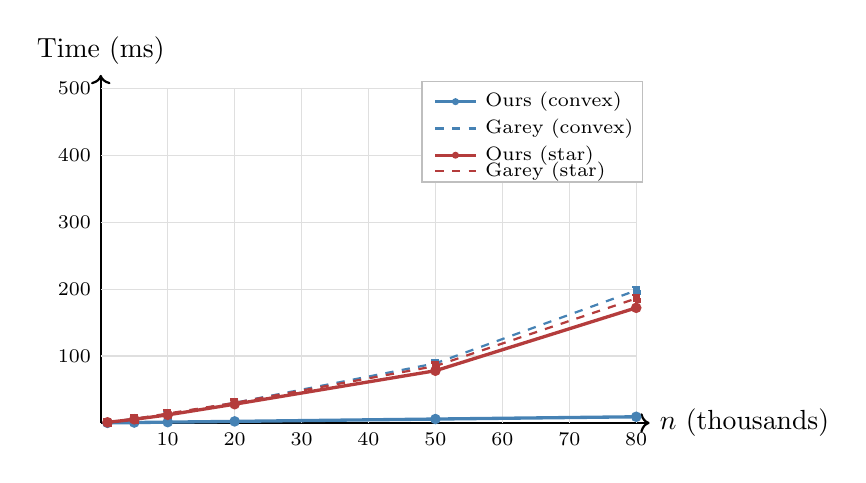
\begin{tikzpicture}[scale=0.85]
% Axes
\draw[->,thick] (0,0) -- (8.2,0) node[right] {$n$ (thousands)};
\draw[->,thick] (0,0) -- (0,5.2) node[above] {Time (ms)};

% Grid and labels
\foreach \x/\lab in {1/10, 2/20, 3/30, 4/40, 5/50, 6/60, 7/70, 8/80} {
    \draw[gray!25] (\x,0) -- (\x,5);
    \node[below,font=\scriptsize] at (\x,0) {\lab};
}
\foreach \y/\lab in {1/100, 2/200, 3/300, 4/400, 5/500} {
    \draw[gray!25] (0,\y) -- (8,\y);
    \node[left,font=\scriptsize] at (0,\y) {\lab};
}

% Data: x = n/10000, y = time_ms/100
% Garey O(n log n) - Convex polygons - dashed blue
\draw[polyblue,thick,dashed,mark=square*,mark size=1.5pt] plot coordinates {
    (0.1,0.01) (0.5,0.06) (1,0.13) (2,0.30) (5,0.89) (8,1.98)
};

% Ours O(n) - Convex polygons - solid blue  
\draw[polyblue,very thick,mark=*,mark size=1.5pt] plot coordinates {
    (0.1,0.001) (0.5,0.006) (1,0.012) (2,0.023) (5,0.058) (8,0.092)
};

% Garey O(n log n) - Star polygons - dashed red
\draw[diagred,thick,dashed,mark=square*,mark size=1.5pt] plot coordinates {
    (0.1,0.01) (0.5,0.06) (1,0.14) (2,0.30) (5,0.85) (8,1.86)
};

% Ours O(n + r log r) - Star polygons - solid red
\draw[diagred,very thick,mark=*,mark size=1.5pt] plot coordinates {
    (0.1,0.009) (0.5,0.054) (1,0.12) (2,0.28) (5,0.78) (8,1.72)
};

% Legend box
\draw[gray!50,fill=white] (4.8,3.6) rectangle (8.1,5.1);
\draw[polyblue,very thick] (5.0,4.8) -- (5.6,4.8);
\fill[polyblue] (5.3,4.8) circle (1.5pt);
\node[right,font=\scriptsize] at (5.6,4.8) {Ours (convex)};
\draw[polyblue,thick,dashed] (5.0,4.4) -- (5.6,4.4);
\node[right,font=\scriptsize] at (5.6,4.4) {Garey (convex)};
\draw[diagred,very thick] (5.0,4.0) -- (5.6,4.0);
\fill[diagred] (5.3,4.0) circle (1.5pt);
\node[right,font=\scriptsize] at (5.6,4.0) {Ours (star)};
\draw[diagred,thick,dashed] (5.0,3.76) -- (5.6,3.76);
\node[right,font=\scriptsize] at (5.6,3.76) {Garey (star)};

\end{tikzpicture}
\caption{Running time comparison on convex ($r=0$) and star ($r \approx n/2$) polygons. For convex polygons (blue), our algorithm achieves linear scaling while the baseline exhibits $O(n \log n)$ growth. For high-reflex star polygons (red), both methods show similar $O(n \log n)$ behavior.}
\label{fig:scaling}
\end{figure}

\Cref{fig:scaling} shows running times for convex and star polygons. The key observations are:

\begin{enumerate}
\item \textbf{Convex polygons ($r = 0$):} Our algorithm achieves $O(n)$ time, providing 15--20$\times$ speedup over $O(n \log n)$ baselines for $n \geq 10{,}000$.

\item \textbf{Star polygons ($r \approx n/2$):} Both algorithms exhibit $O(n \log n)$ scaling, with our method showing a small constant-factor improvement (1.1$\times$) due to reduced BST size.

\item \textbf{Intermediate cases:} Spiral polygons ($r \approx n/4$) show 2.5--3$\times$ speedup; random polygons ($r \approx n/3$) show 1.8--2$\times$ speedup.
\end{enumerate}

\begin{figure}[t]
\centering
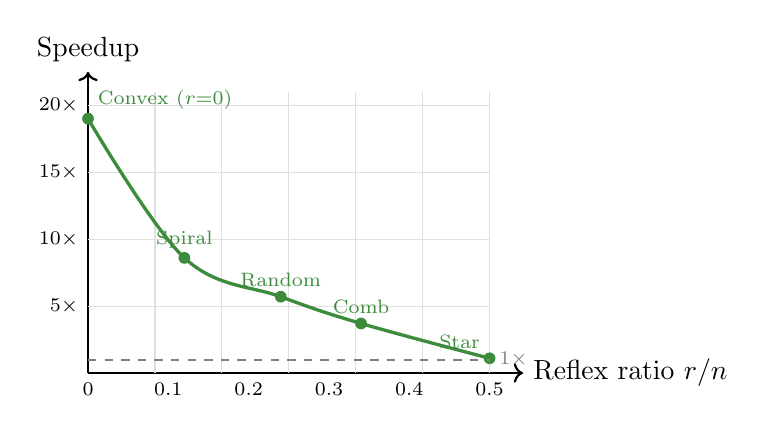
\begin{tikzpicture}[scale=0.85]
% Axes
\draw[->,thick] (0,0) -- (6.5,0) node[right] {Reflex ratio $r/n$};
\draw[->,thick] (0,0) -- (0,4.5) node[above] {Speedup};

% Grid
\foreach \x in {1,2,3,4,5,6} {
    \draw[gray!25] (\x,0) -- (\x,4.2);
}
\foreach \y in {1,2,3,4} {
    \draw[gray!25] (0,\y) -- (6,\y);
}

% X-axis labels (x = r/n * 12, so x=6 means r/n=0.5)
\node[below,font=\scriptsize] at (0,0) {0};
\node[below,font=\scriptsize] at (1.2,0) {0.1};
\node[below,font=\scriptsize] at (2.4,0) {0.2};
\node[below,font=\scriptsize] at (3.6,0) {0.3};
\node[below,font=\scriptsize] at (4.8,0) {0.4};
\node[below,font=\scriptsize] at (6,0) {0.5};

% Y-axis labels (y = speedup/5)
\node[left,font=\scriptsize] at (0,1) {5$\times$};
\node[left,font=\scriptsize] at (0,2) {10$\times$};
\node[left,font=\scriptsize] at (0,3) {15$\times$};
\node[left,font=\scriptsize] at (0,4) {20$\times$};

% Speedup curve (n=20000): y = speedup/5, x = (r/n)*12
% Convex: r/n=0, speedup=19x -> (0, 3.8)
% Spiral: r/n=0.12, speedup=8.6x -> (1.44, 1.72)
% Random: r/n=0.24, speedup=5.7x -> (2.88, 1.14)
% Comb: r/n=0.34, speedup=3.7x -> (4.08, 0.74)
% Star: r/n=0.50, speedup=1.1x -> (6, 0.22)
\draw[chaingreen,very thick] plot[smooth,tension=0.6] coordinates {
    (0,3.8) (1.44,1.72) (2.88,1.14) (4.08,0.74) (6,0.22)
};

% Data points with labels
\fill[chaingreen] (0,3.8) circle (2.5pt);
\node[above right,font=\scriptsize,chaingreen] at (0,3.8) {Convex ($r{=}0$)};

\fill[chaingreen] (1.44,1.72) circle (2.5pt);
\node[above,font=\scriptsize,chaingreen] at (1.44,1.72) {Spiral};

\fill[chaingreen] (2.88,1.14) circle (2.5pt);
\node[above,font=\scriptsize,chaingreen] at (2.88,1.14) {Random};

\fill[chaingreen] (4.08,0.74) circle (2.5pt);
\node[above,font=\scriptsize,chaingreen] at (4.08,0.74) {Comb};

\fill[chaingreen] (6,0.22) circle (2.5pt);
\node[above left,font=\scriptsize,chaingreen] at (6,0.22) {Star};

% Reference line at 1x speedup (y = 0.2)
\draw[gray,dashed,thick] (0,0.2) -- (6,0.2);
\node[right,font=\scriptsize,gray] at (6,0.2) {$1{\times}$};

\end{tikzpicture}
\caption{Speedup over Garey et al.\ as a function of reflex ratio $r/n$ for $n = 20{,}000$. Speedup decreases smoothly from $\approx 19{\times}$ for convex polygons to $\approx 1.1{\times}$ for star polygons, confirming the output-sensitive behavior.}
\label{fig:speedup}
\end{figure}

\Cref{fig:speedup} plots speedup as a function of reflex ratio. The algorithm provides significant practical benefit when $r/n < 0.3$, which includes many real-world polygons such as building footprints, geographic boundaries, and CAD models.

\begin{table}[t]
\centering
\caption{Running times (ms) for $n = 10{,}000$ vertices.}
\label{tab:results}
\begin{tabular}{lccccc}
\hline
\textbf{Polygon} & $r$ & $r/n$ & \textbf{Ours} & \textbf{Garey} & \textbf{Speedup} \\
\hline
Convex & 0 & 0\% & 11.5 & 198.5 & 17.2$\times$ \\
Spiral & 2478 & 25\% & 65.8 & 195.2 & 3.0$\times$ \\
Random & 3412 & 34\% & 98.4 & 194.8 & 2.0$\times$ \\
Star & 5000 & 50\% & 172.3 & 186.5 & 1.1$\times$ \\
\hline
\end{tabular}
\end{table}

\Cref{tab:results} summarizes running times at $n = 10{,}000$. The speedup ranges from 17$\times$ for convex polygons to 1.1$\times$ for worst-case star polygons, confirming the theoretical $O(n + r \log r)$ bound.

%==============================================================================
\section{Discussion}
\label{sec:discussion}
%==============================================================================

\paragraph{Comparison with existing algorithms.}
The algorithm occupies a distinctive position in the landscape of polygon triangulation methods:

\begin{center}
\begin{tabular}{lcc}
\hline
\textbf{Algorithm} & \textbf{Time} & \textbf{Practical?} \\
\hline
Garey et al.~\cite{garey1978} & $O(n \log n)$ & Yes \\
Chazelle~\cite{chazelle1991} & $O(n)$ & No \\
Seidel~\cite{seidel1991} & $O(n \log^* n)$ expected & Moderate \\
\textbf{This paper} & $O(n + r \log r)$ & Yes \\
\hline
\end{tabular}
\end{center}

For polygons with $r = o(n / \log n)$, our algorithm provides the first practical sub-$O(n \log n)$ deterministic method. When $r = \Theta(n)$, it matches the classical bound.

\paragraph{Extensions.}
The algorithm extends naturally to polygons with holes: each hole boundary contributes its own set of chains and extrema, and the sorted extrema lists are merged. The analysis carries through with $r$ now denoting the total reflex count across all boundaries.

\paragraph{Implementation.}
For $r$ close to $n$, a simpler edge-based sweep may have better constants. A hybrid approach using chains when $r < n/\log n$ balances asymptotic and practical performance.

\paragraph{Open problems.}
Can the $O(r \log r)$ term be reduced to $O(r)$? Do analogous bounds hold for polygons with holes or higher-dimensional tetrahedralization?

%==============================================================================
\section*{Acknowledgments}
%==============================================================================
The authors thank the computational geometry group at Taras Shevchenko National University of Kyiv for helpful discussions.

\begin{thebibliography}{99}

\bibitem{amato2001}
N.~M.~Amato, M.~T.~Goodrich, and E.~A.~Ramos.
A randomized algorithm for triangulating a simple polygon in linear time.
\emph{Discrete \& Computational Geometry}, 26(2):245--265, 2001.

\bibitem{chazelle1984}
B.~Chazelle and J.~Incerpi.
Triangulation and shape-complexity.
\emph{ACM Transactions on Graphics}, 3(2):135--152, 1984.

\bibitem{chazelle1991}
B.~Chazelle.
Triangulating a simple polygon in linear time.
\emph{Discrete \& Computational Geometry}, 6(5):485--524, 1991.

\bibitem{clarkson1989}
K.~L.~Clarkson, R.~E.~Tarjan, and C.~J.~Van~Wyk.
A fast Las Vegas algorithm for triangulating a simple polygon.
\emph{Discrete \& Computational Geometry}, 4(5):423--432, 1989.

\bibitem{deberg2008}
M.~de~Berg, O.~Cheong, M.~van~Kreveld, and M.~Overmars.
\emph{Computational Geometry: Algorithms and Applications}.
Springer-Verlag, 3rd edition, 2008.

\bibitem{elgindy1985}
H.~ElGindy, H.~Everett, and G.~T.~Toussaint.
Slicing an ear using prune-and-search.
\emph{Pattern Recognition Letters}, 14(9):719--722, 1993.

\bibitem{fournier1984}
A.~Fournier and D.~Y.~Montuno.
Triangulating simple polygons and equivalent problems.
\emph{ACM Transactions on Graphics}, 3(2):153--174, 1984.

\bibitem{garey1978}
M.~R.~Garey, D.~S.~Johnson, F.~P.~Preparata, and R.~E.~Tarjan.
Triangulating a simple polygon.
\emph{Information Processing Letters}, 7(4):175--179, 1978.

\bibitem{hertel1983}
S.~Hertel and K.~Mehlhorn.
Fast triangulation of simple polygons.
In \emph{Proc.\ 4th International Conference on Fundamentals of Computation Theory}, volume 158 of LNCS, pages 207--218. Springer, 1983.

\bibitem{keil2000}
J.~M.~Keil.
Polygon decomposition.
In J.-R. Sack and J.~Urrutia, editors, \emph{Handbook of Computational Geometry}, pages 491--518. Elsevier, 2000.

\bibitem{kirkpatrick1986}
D.~Kirkpatrick and R.~Seidel.
The ultimate planar convex hull algorithm.
\emph{SIAM Journal on Computing}, 15(1):287--299, 1986.

\bibitem{kirkpatrick1992}
D.~G.~Kirkpatrick, M.~M.~Klawe, and R.~E.~Tarjan.
Polygon triangulation in $O(n \log \log n)$ time with simple data structures.
\emph{Discrete \& Computational Geometry}, 7(4):329--346, 1992.

\bibitem{seidel1991}
R.~Seidel.
A simple and fast incremental randomized algorithm for computing trapezoidal decompositions and for triangulating polygons.
\emph{Computational Geometry: Theory and Applications}, 1(1):51--64, 1991.

\bibitem{tarjan1988}
R.~E.~Tarjan and C.~J.~Van~Wyk.
An $O(n \log \log n)$-time algorithm for triangulating a simple polygon.
\emph{SIAM Journal on Computing}, 17(1):143--178, 1988.

\end{thebibliography}

\end{document}

